\hypertarget{course1}{}\chapter*{COURSE 1: Self-Awareness}\label{course1}
\addcontentsline{toc}{chapter}{COURSE 1: Self-Awareness}
\extramarks{ }{COURSE 1: Self-Awareness}

\noindent\makebox[\textwidth]{\rule{\linewidth}{0.4pt}}
\localtableofcontents
\noindent\makebox[\textwidth]{\rule{\linewidth}{0.4pt}}
\pagebreak \section*{Module 1: Networking: Why and How}\addcontentsline{toc}{section}{Module 1: Networking: Why and How} \extramarks{Module 1}{COURSE 1: Self-Awareness}
\noindent\makebox[\textwidth]{\rule{\linewidth}{0.4pt}} \etocsetnexttocdepth{4}
\localtableofcontents
\noindent\makebox[\textwidth]{\rule{\linewidth}{0.4pt}}

\leftskip=0.5cm
We all have different kinds of relationships with people: casual, familial, professional, intimate, etc. Throughout our lives, these relationships provide us with different types of support. Your parents, siblings, teachers, doctors, employers, coworkers, and even bus or taxi drivers are all part of your personal network of relationships.

Because most job seekers get hired through a personal connection of one sort or another, knowing who is in your network is extremely important to your job search. Throughout this course you will be asked to seek information, guidance, and advice from your network, so it's important to properly define and organize your relationships.

\pagebreak \subsection*{1-1\quad The Network Pyramid}
\addcontentsline{toc}{subsection}{1-1\quad The Network Pyramid}
A good way of organizing your network is to use the shape of a five-level pyramid, starting with a narrow peak at the top and broadening to a large base at the bottom. Each level of the pyramid contains a different group of people, based on their closeness to you.

\subsubsection*{The First Level (top of the pyramid or the point of the pyramid)}

Since your personal network pyramid organizes relationships as they relate to you, the top level belongs to you alone. As the pyramid broadens toward the base, the levels also get further away from you at the top. Keep this in mind as you fill in the rest of the pyramid.

\subsubsection*{The Second Level (second from the top of the pyramid or fourth from the bottom)}

Level two contains the people with whom you are closest. You might include your parents, close siblings, spouse, boyfriend or girlfriend, religious leaders you have come to know well, and very close friends. These are the people you feel comfortable sharing most of your thoughts and feelings, knowing any sensitive information would be treated confidentially.

\subsubsection*{The Third Level (the middle level of the pyramid)}

Most of your friends, classmates, coworkers, and people with whom you often interact will be in the third level. This level is for established friends and solid relationships. Extended family members you enjoy spending time with are appropriate for this level as well.

\subsubsection*{The Fourth Level (second level from the bottom)}

The fourth level is the place for acquaintances. Some examples are a former or current classmate, a neighbor, or a coworker.

\subsubsection*{The Fifth Level (bottom level and widest level or base of the pyramid)}

The fifth level of your network pyramid represents people you rarely encounter. Here is where to place people you pay to assist you, your doctors, dentist, and hairdresser, or people who help you with shopping or transportation needs. The people here are not strangers, but they are also not likely to become your friends.

To use this networking pyramid, we will focus on identifying a professional mentor within these levels. We will look for someone who aligns with your career goals, shares their expertise, and can provide professional guidance. Remember, mentors don’t have to be strangers; they can be established connections who genuinely care about your growth and success. Seek out those who inspire you and are willing to invest in your professional development.
\clearpage
\mbox{}
\vfill 
\begin{figure}[!ht]
    \centering
    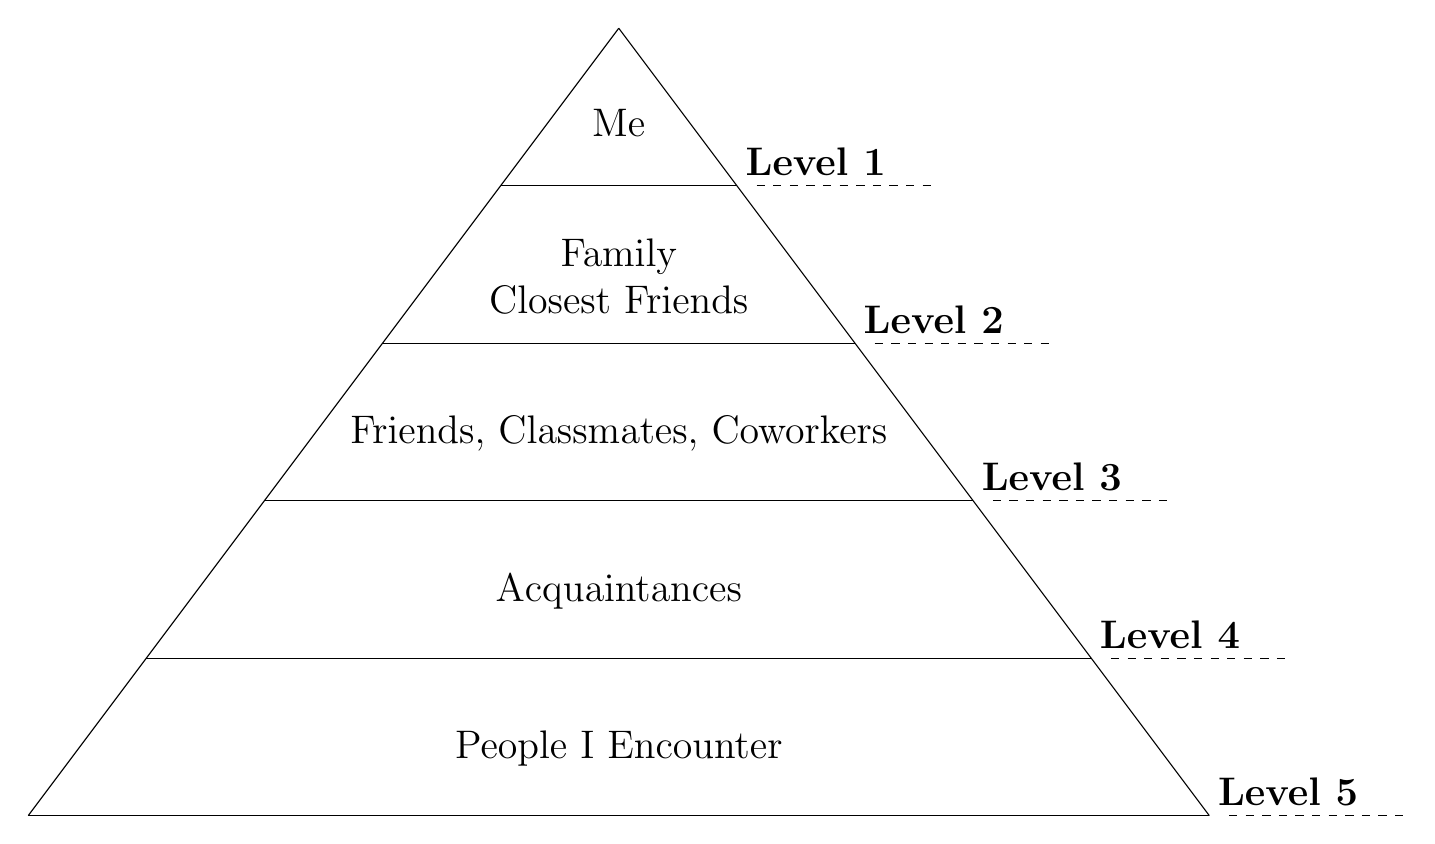
\begin{tikzpicture}[scale=1]
        \def\h{10}; % Height of the pyramid
        \def\f{.75}; % Factor to control the width of each layer
        
        % Draw the horizontal lines for each layer
        \foreach \y in {0,2,4,6,8} {
            \def\w{\h*\f-\y*\f};
            \def\v{\y*\f-\h*\f};
            \draw (\v,\y) -- (\w,\y);
        }
        \draw[dashed] (7.75,0) -- (10,0);
        \draw[dashed] (6.25,2) -- (8.5,2);
        \draw[dashed] (4.75,4) -- (7,4);
        \draw[dashed] (3.25,6) -- (5.5,6);
        \draw[dashed] (1.75,8) -- (4,8);

        
        % Draw the vertical lines for the sides
        \draw (-\h*\f,0) -- (0,\h);
        \draw (\h*\f,0) -- (0,\h);
        
        % Label each layer
        \node at (0,0.5) [above] {\Large People I Encounter};
        \node at (0,2.5) [above] {\Large Acquaintances};
        \node at (0,4.5) [above] {\Large Friends, Classmates, Coworkers};
        \node at (0,6.75) [above] {\Large Family};
        \node at (0,6.25) [above] {\Large Closest Friends};
        \node at (0,8.5) [above] {\Large Me};
        \node at (8.5,0) [above] {\Large \textbf{Level 5}};
        \node at (7,2) [above] {\Large \textbf{Level 4}};
        \node at (5.5, 4) [above] {\Large \textbf{Level 3}};
        \node at (4,6) [above] {\Large \textbf{Level 2}};
        \node at (2.5,8) [above] {\Large \textbf{Level 1}};
    \end{tikzpicture}
    \caption{Image of Pyramid with 5 Levels from 1st Level at the tip of the pyramid to 5th at its base}
\end{figure}
\mbox{}
\vfill{}
\clearpage


\pagebreak \subsection*{1-2\quad Assignment: Your Network Pyramid}
\addcontentsline{toc}{subsection}{1-2\quad Assignment: Your Network Pyramid}
Read the APH CareerConnect article, \href{https://aphconnectcenter.org/careerconnect-blog/networking-your-way-to-becoming-a-brave-and-brilliant-professional/}{Game On: Networking Your Way to Becoming a Brave and Brilliant Professional}.

Write out who is included in your network pyramid, starting with you at the top level (level one) and filling in the names of your intimates (level two), friends (level three), acquaintances (level four), and paid helpers or casual acquaintances (level five).

\pagebreak \subsection*{1-3\quad Example Assignment: Denise's Network Pyramid}
\addcontentsline{toc}{subsection}{1-3\quad Example Assignment: Denise's Network Pyramid}
\subsubsection*{First Level (Top Level):}
\begin{itemize}[leftmargin=1.0cm]
	\item Me (Denise)
\end{itemize}

\subsubsection*{Second Level:}
\begin{multicols}{2}
	\begin{itemize}[leftmargin=1.0cm]
		\item Parents
		\item Jason  \break(younger brother)
		\item Katie  \break(older sister)
		\item Matt  \break(brother in-law)
		\item Laverne  \break(sister in- law)
		\item Freddie
		\item Nicolas
		\item George
		\item James and Lisa \break(nephews and niece)
		\item Jacob
		\item Jack
		\item Tim
		\item Tina
		\item Olga
		\item Nicole
		\item Jessica \break(cousins)
		\item Mark
		\item Dave
		\item Amy
		\item Tiffany
		\item Jamie
		\item Collin
		\item Ryan  \break(best friend)
	\end{itemize}
\end{multicols}
\pagebreak \subsubsection*{Third Level:}
\begin{multicols}{2}
	\begin{itemize}[leftmargin=1.0cm]
		\item Jenny
		\item Tiffany V.
		\item Sherlanda
		\item Jermaine
		\item Jacky
		\item Meghan
		\item Monica
		\item Jeremy
		\item Jason
		\item Vinnie
		\item Carl
		\item Paul
		\item Johnny
		\item Cindy
		\item Heather
		\item Helen
		\item Tim
		\item Chris
		\item Kevin
		\item Rick
		\item Jim
		\item Hillary
		\item Hal
		\item Harvey
		\item Sean
		\item Lauren
		\item Tilly
		\item Tori
		\item Sarah
		\item Christi
		\item Audrey
		\item Elizabeth
		\item Vicky
		\item Sonya and Joan \break(classmates and friends)
	\end{itemize}
\end{multicols}
\pagebreak  \subsubsection*{Fourth Level:}
\begin{multicols}{2}
	\begin{itemize}[leftmargin=1.0cm]
		\item Mrs. Barbieri
		\item Ms. Tiffany
		\item Mr. Columbus
		\item Mr. Salvador
		\item Miss Bogota
		\item Miss Frost
		\item Mr. Turkeyham \break(teacher I am close to)
		\item Courtney
		\item Sarah
		\item Jeremy
		\item Jack
		\item Josh
		\item George
		\item Billy
		\item Kevin
		\item Mike
		\item Andy
		\item Jon
		\item Darren
		\item Andrew
		\item Barbie
		\item Jackie
		\item Roxy
		\item Rebecca
		\item Janet
		\item Georgia
		\item Amy
		\item Jane
		\item Jessica
		\item Fred
		\item Tom
		\item Manny
		\item Chenoa
		\item Casey
		\item Cassandra
		\item Jennifer and Jenna \break(people I have met at school and at the community center and who I like but are not yet friends)
	\end{itemize}
\end{multicols}
\pagebreak \subsubsection*{Fifth Level:}
\begin{multicols}{2}
	\begin{itemize}[leftmargin=1.0cm]
		\item Dr. Susan Carrotosis \break(ophthalmologist)
		\item Mr. Tom \break(cafeteria worker)
		\item Mrs. Jacobs
		\item Mr. Franklin
		\item Mr. South
		\item Miss Jonas
		\item Ms. Frascator
		\item Coach Longo
		\item Mr. Sean Combs
		\item Ms. Ray
		\item Mr. Benny
		\item Ms. Malik \break(teachers)
		\item Mr. Freise \break(Principal of my high school)
		\item Andre \break(taxi driver)
		\item Tara \break(bike store clerk)
		\item Silvio \break(pizza guy)
		\item Jack \break(landscaper)
		\item Jim \break(ice cream shop clerk)
		\item Ed \break(physical therapist)
		\item Jenny \break(religious schoolteacher)
		\item Mr. Nick Afflitto \break(drum teacher)
		\item Mr. Michaels \break(family doctor)
		\item Ms. Denise \break(nurse)
		\item Mrs. Jennings \break(dentist)
		\item Jeff \break(supermarket customer service representative)
		\item Ms. Jacky \break(librarian)
		\item Frank  \break(handyman in my apartment building).
	\end{itemize}
\end{multicols}

The assignment associated with this module is available in the \href{#course1workbook}{Course 1 Workbook, Module 1-2}.

\pagebreak \section*{Module 2: Building, Expanding and Maintaining Your Network}\addcontentsline{toc}{section}{Module 2: Building, Expanding and Maintaining Your Network}\extramarks{Module 2}{COURSE 1: Self-Awareness}
\noindent\makebox[\textwidth]{\rule{\linewidth}{0.4pt}} \etocsetnexttocdepth{4}
\localtableofcontents
\noindent\makebox[\textwidth]{\rule{\linewidth}{0.4pt}}


\pagebreak \subsection*{2-1\quad Lesson: Developing contacts that can help provide employment opportunities}
\addcontentsline{toc}{subsection}{2-1\quad Lesson: Developing contacts that can help provide employment opportunities}
All relationships offer some sort of benefit, whether it's friendship, knowledge, or simply a chance to know someone new. A network is a supportive system made up of these relationships, built around sharing information and services among individuals who have a common interest or connection.

Networking means to be actively cultivating relationships with people who might be helpful to you professionally, either in finding employment or moving to a higher position. Networking is an important skill particularly for an active job seeker. Just like any other skill, becoming a good networker requires much practice. Many opportunities to network will present themselves in your daily life, you just need to identify and act on them.

\subsubsection*{Building a Professional Network}
Building a strong professional network can significantly enhance your career growth and provide valuable guidance. Here are some strategies to connect with potential mentors:

\subsubsection*{Industry Events and Conferences:}
   Attend conferences, workshops, and industry-specific events. These gatherings bring together professionals who share common interests. Engage in conversations, ask questions, and express your eagerness to learn. Look for experienced individuals who resonate with your career goals.

\subsubsection*{Online Platforms and Forums:}
   Explore online platforms like LinkedIn, industry-specific forums, and professional groups. Join relevant discussions, contribute insights, and connect with professionals in your field. Be genuine in your interactions and express your interest in mentorship.

\subsubsection*{Alumni Networks:}
   Leverage your educational institution's alumni network. Alumni often have a strong desire to support fellow graduates. Attend alumni events, reach out to alumni working in your desired field, and express your interest in mentorship.

\subsubsection*{Professional Associations:}
   Join professional associations related to your industry. Attend their meetings, workshops, and networking events. These associations often have mentorship programs or can connect you with experienced professionals willing to guide you.

\subsubsection*{Cold Outreach:}
   Don't hesitate to reach out directly to professionals you admire. Craft a thoughtful email or message explaining your interest in their work and your desire for mentorship. Be respectful of their time and express gratitude for any guidance they provide.

\subsubsection*{Volunteer Work and Nonprofits:}
   Engage in volunteer activities related to your field. Volunteering exposes you to like-minded individuals and potential mentors. Nonprofit organizations often have passionate professionals who are open to mentoring.

\subsubsection*{Informal Coffee Chats:}
   Invite professionals for casual coffee chats. Use these opportunities to learn about their career journey, seek advice, and express your interest in mentorship. Remember to be respectful and appreciative of their time.

Remember, mentorship is a two-way street. Be open to learning, actively listen, and show appreciation for the insights shared by your mentor. Building authentic relationships will not only help you find suitable work but also accelerate your professional growth.

\subsubsection*{Cultivating Meaningful Professional Connections}
Cultivating meaningful connections with mentors can significantly impact your personal and professional growth. Here are some strategies to foster mentor relationships:

\subsubsection*{Genuine Curiosity:}
\begin{itemize}[leftmargin=1.0cm]
\item Approach mentorship with a sincere desire to learn from others. Be genuinely curious about their experiences, insights, and expertise.
\item Ask open-ended questions that allow them to share their knowledge and wisdom.
\end{itemize}
\subsubsection*{Active Listening:}
\begin{itemize}[leftmargin=1.0cm]
\item When interacting with mentors, actively listen to what they say. Pay attention to their stories, challenges, and triumphs.
\item Show empathy and understanding. Acknowledge their perspectives and experiences.
\end{itemize}
\subsubsection*{Share Your Journey:}
\begin{itemize}[leftmargin=1.0cm]
\item While it's essential to be curious about your mentor's life, don't hesitate to share your own journey. Be authentic and transparent.
\item Discuss your goals, aspirations, and any obstacles you're facing. Mentors appreciate vulnerability.
\end{itemize}
\subsubsection*{Regular Check-Ins:}
\begin{itemize}[leftmargin=1.0cm]
\item Maintain regular communication with your mentors. It's not about quantity but consistency.
\item Send occasional updates via email or schedule brief catch-up calls. Share your progress and seek their guidance.
\end{itemize}
\subsubsection*{Remember Details:}
\begin{itemize}[leftmargin=1.0cm]
\item Keep a record of your interactions. Create a file with notes about what you've discussed with each mentor.
\item Include personal details, career advice, and any specific insights they've shared. This helps you recall important information.
\end{itemize}
\subsubsection*{Acknowledge Their Impact:}
\begin{itemize}[leftmargin=1.0cm]
\item Express gratitude for their mentorship. Let them know how their guidance has influenced your decisions and growth.
\item A simple thank-you note or message goes a long way.
\end{itemize}
\subsubsection*{Be Respectful of Their Time:}
\begin{itemize}[leftmargin=1.0cm]
\item When reaching out, be mindful of their busy schedules. Respect their time and availability.
\item If you have a specific question or need advice, be concise and focused.
\end{itemize}
Remember, mentorship is a reciprocal relationship. Show appreciation, be open to learning, and invest in building authentic connections.

\subsubsection*{Social Networking: Pros and Cons}
Certainly! Let's explore the pros and cons of using social media Social networking platforms like Facebook, Instagram, LinkedIn, TikTok and Twitter (also called ``X'') offer both opportunities and challenges for job seekers. Here's a balanced perspective:

\subsubsection*{Advantages of Using Social Media for Job Hunting:}
\begin{enumerate}[leftmargin=1cm]
\item Efficient and Convenient:
\begin{itemize}[leftmargin=1cm]
   \item Social media allows you to search for jobs effortlessly. Mobile apps provide push notifications, ensuring you don't miss updates from your professional network.
   \item You can express interest in job opportunities directly through platforms like Facebook groups or LinkedIn messages.
   \end{itemize}
\item Establishes Professional Connections:
\begin{itemize}[leftmargin=1cm]
   \item Use social media to build relationships with busy professionals, including business owners, content creators, and recruiters.
   \item Share your expertise, engage with their content, and connect meaningfully.
   \end{itemize}
\item Increases Visibility:
\begin{itemize}[leftmargin=1cm]
   \item Over **4.26 billion** people use social media, and this number is growing. Recruiters and CEOs are active on these platforms.
   \item Friends in your network can share your job-seeking posts or guide you to relevant opportunities.
   \end{itemize}
\item Little to No Cost:
\begin{itemize}[leftmargin=1cm]
   \item Social media is a cost-effective way to expand your job search. Both job seekers and employers benefit without significant expenses.
   \end{itemize}
   \end{enumerate}
\subsubsection*{Disadvantages of Using Social Media for Job Hunting:}
\begin{enumerate}[leftmargin=1cm]
\item Public Exposure:
\begin{itemize}[leftmargin=1cm]
   \item Employers often review social media profiles during the hiring process. Assume that anything you post is visible to potential employers.
   \item What seems like a harmless joke to friends might appear unprofessional or irresponsible to a hiring manager.
   \end{itemize}
\item Privacy Concerns:
\begin{itemize}[leftmargin=1cm]
   \item Despite privacy settings, you have limited control over shared content. Assume that everything you post could impact your professional image.
   \item Be cautious about personal posts, controversial opinions, or inappropriate content.
   \end{itemize}
\item Competition and Noise:
\begin{itemize}[leftmargin=1cm]
   \item Everyone has access to the same social media platforms. Job postings can get lost in the noise.
   \item Balancing visibility with maintaining a professional image is crucial.
   \end{itemize}
\end{enumerate}
\subsubsection*{Strategies for Effective Social Media Job Hunting:}
\begin{enumerate}[leftmargin=1cm]
\item Optimize Your Profiles:
\begin{itemize}[leftmargin=1cm]
\item Update your LinkedIn profile with relevant keywords, a professional photo, and a compelling summary.
\item Showcase your skills, accomplishments, and career aspirations.
\end{itemize}
\item Network Actively:
\begin{itemize}[leftmargin=1cm]
   \item Engage with industry-specific groups, follow thought leaders, and participate in discussions.
   \item Connect with professionals who inspire you and seek mentorship.
\end{itemize}
\item Curate Your Content:
\begin{itemize}[leftmargin=1cm]
   \item Share industry insights, articles, and relevant news. Demonstrate your expertise.
   \item Avoid controversial topics or offensive language.
\end{itemize}
\item Monitor Your Online Presence:
\begin{itemize}[leftmargin=1cm]
   \item Regularly review your social media profiles. Remove any content that doesn't align with your professional image.
   \item Google your name to see what potential employers might find.
   \end{itemize}
   \end{enumerate}

Remember, social media can be a powerful ally in your job search if used strategically. Balance authenticity with professionalism, and leverage these platforms to enhance your career prospects. 

Read the APH CareerConnect article, \href{https://aphconnectcenter.org/careerconnect-blog/how-can-linkedin-benefit-the-job-seeker-who-is-blind-or-low-vision/}{How can LinkedIn Benefit the Visually Impaired Job Seeker?}

\subsubsection*{Key Take-away:}
\subsubsection*{Never Stop Networking!}

Even if you currently have a job, continue to expand and maintain your network. Getting a better job is easier if you're currently employed. Additionally, if you keep active with your network, your contacts will be more likely to think about you when an opportunity arises.


\pagebreak \subsection*{2-2\quad Assignment: Your Network Expansion Plan}
\addcontentsline{toc}{subsection}{2-2\quad Assignment: Your Network Expansion Plan}
Read the APH CareerConnect article, \href{https://aphconnectcenter.org/careerconnect-blog/principles-for-expanding-your-professional-network-when-you-are-blind-or-low-vision/}{Principles for Expanding Your Professional Network When You are Blind or Visually Impaired}.

In a paragraph or two, outline your strategy for expanding your professional network. Will you be joining any organizations or groups? If so, which ones, and how do you anticipate that joining will enhance your career growth? Additionally, consider how the information in this paragraph can guide your criteria for selecting a mentor. What qualities or expertise would you seek in a mentor to support your professional development?

\pagebreak \subsection*{2-3\quad Example Assignment: Darlene's Network Expansion Plan}
\addcontentsline{toc}{subsection}{2-3\quad Example Assignment: Darlene's Network Expansion Plan}
I plan to join the organization Distributive Education Cooperative of America (DECA) at school. DECA participates in marketing competitions at the regional and state levels. I have been taking a few business courses at my high school and DECA utilizes the skills we learn in those classes.
The organization gives the chance to network with other students from my school and from schools throughout the state and possibly country. I'll also get to meet professionals from the field of marketing who serve as judges. There is also a possibility of winning scholarships to post-secondary schools. Joining DECA will allow me to showcase my skills in business and network with students and professionals interested in the same occupational field.

There is another organization called Future Business Leaders of America (FBLA) that I can join. The focus is more on general business strategies, skills and structures of business. Both organizations will be important in expanding my personal network.

\pagebreak \section*{Module 3:	Self-Assessment and Constructive Feedback}\addcontentsline{toc}{section}{Module 3:	Self-Assessment and Constructive Feedback}\extramarks{Module 3}{COURSE 1: Self-Awareness}
\noindent\makebox[\textwidth]{\rule{\linewidth}{0.4pt}} \etocsetnexttocdepth{4}
\localtableofcontents
\noindent\makebox[\textwidth]{\rule{\linewidth}{0.4pt}}

\pagebreak \subsection*{3-1\quad Lesson: Identifying your strengths and weaknesses through constructive criticism}
\addcontentsline{toc}{subsection}{3-1\quad Lesson: Identifying your strengths and weaknesses through constructive criticism}
\subsubsection*{The Self-Assessment}
Self-assessment is a process of careful reflection, discovery, and analysis in order to articulate your strengths, weaknesses, interests, skills, abilities, values, personality, and goals.

Performing a self-assessment at the beginning of your career exploration is important for many reasons. A thorough self-assessment will help you focus your job search and preparation on those positions that hold the most appeal to you and are the best match for your skills. Self-assessment identifies the areas about which you can be confident in your abilities and the areas where you might want to work on improvement. Maybe more important, self-assessment helps you articulate your goals and aspirations, so you know what you're working toward both in the long- and short-term.

\subsubsection*{Seeking feedback from others}
The first step in your self-assessment is to seek feedback in the form of constructive criticism from people you know and trust.

\subsubsection*{Why feedback?}
Job market applicants are often judged by their presentation. The image you project to a potential employer often makes up a great deal of the information he or she will consider about you. It's important to get a good sense of how you are perceived by others so you can emphasize your strengths, improve your weaknesses, and take control of your image. In order for you to know how others see you, and what you might want to adjust, you need to ask for constructive criticism.

\subsubsection*{Constructive criticism}
All of us need help and a variety of opinions when determining how we are seen by the people in our lives. Those who can best help us see ourselves objectively are the people with whom we interact most. In your assignment for this lesson, you will be asking a variety of people you know for their honest opinions of both your strengths and weaknesses. The goal of this exercise is to get an objective and accurate understanding of how you present yourself to the world.

The kind of feedback you will seek is called constructive criticism. The purpose of constructive criticism is not to make you feel bad or to focus on your flaws, but to celebrate your assets and identify those areas you might want to improve or change.

Knowing both your strengths and weaknesses can be a valuable tool for improvement. While it's always nice to hear what people think of as our strengths, it can be challenging to hear what people think of as our weaknesses. Focus on using this information to your advantage. Analyze each person's opinion, then take a good look to see how you can improve on the areas they've mentioned. Try to avoid becoming defensive when someone offers an honest opinion, even if it differs from your own. Remember that this is a self-enrichment exercise. Being open and available to constructive criticism can really help you develop and mature as an individual.

Read the APH CareerConnect article, \href{https://aphconnectcenter.org/self-advocacy/negative-feedback-how-to-handle-it-and-how-to-use-it/}{Negative Feedback: How to Handle it and How to Use It}.

\subsubsection*{Choosing your participants}
When you're thinking of people to ask for constructive criticism, remember that you want a range of opinions from people involved in different aspects of your life. Ideally, some people you ask will know you very well, like family members or close friends, and others will be familiar with you, but not intimate. Refer to your network pyramid: choose people from levels two, three, and four to get a good variety of opinions.

Remember that you are asking these people for their help and their time. Before asking someone for an opinion, take some time to think about how you will present yourself when you ask. If you are just coming back from the gym and haven't showered yet, this might have an effect on how you are perceived, and it also might not be the best example of how you would present yourself to a potential employer. Take the time to present yourself in a realistic light so that the person you're asking for help can offer feedback that is useful and relevant.
\pagebreak \subsection*{3-2\quad Assignment: Feedback}
\addcontentsline{toc}{subsection}{3-2\quad Assignment: Feedback}
\subsubsection*{Part 1: Constructive Criticism}

During the next two days ask five different people (family members, friends, classmates, teachers, former co- workers, or others) for feedback about you. Ask each participant to provide 5 to 10 comments that describe you, balanced between strengths and weaknesses: the things they think you do well and those that could use improvement. Collect responses digitally; you'll be using them later. Be sure to include the name of the respondent and their relationship to you.
\subsubsection*{Part 2: Analysis}

Compile a list of the strengths and weaknesses you heard in your feedback. Describe what you liked hearing and what you did not like hearing. When listing areas for improvement, think about how you might go about making changes.
\pagebreak \subsection*{3-3\quad Example Assignment: Debbie's Feedback Notes}
\addcontentsline{toc}{subsection}{3-3\quad Example Assignment: Debbie's Feedback Notes}
\subsubsection*{Part 1: Constructive Criticism}
\subsubsection*{Feedback from: Mother}
\begin{itemize}[leftmargin=1.0cm]
	\item Pretty hair
	\item Caring
	\item Organized
	\item Talkative, which can either be a good or a bad thing
	\item Well read, reads a lot
	\item Good with animals
	\item Dresses well
	\item Sometimes dozes off at inappropriate times
	\item Helpful at home
	\item Impatient at times
\end{itemize}
\subsubsection*{Feedback from: Mrs. Smith, English teacher}
\begin{itemize}[leftmargin=1.0cm]
	\item Good technology skills
	\item Usually organized
	\item Well dressed
	\item Excellent reader
	\item Has a tendency to procrastinate
	\item Gets along with classmates
	\item Enthusiastic
	\item Tends to monopolize conversations
	\item Impatient
	\item Shy in new situations, takes time to become comfortable
\end{itemize}
\subsubsection*{Feedback from Mary, older sister}
\begin{itemize}[leftmargin=1.0cm]
	\item Smart
	\item Reads a lot
	\item Nice
	\item Clean
	\item Good sister
	\item Talks a lot
	\item Good on the computer
	\item Opinionated at times
	\item Takes over conversations and interrupts
\end{itemize}
\subsubsection*{Feedback from Jana, friend and fellow club member}
\begin{itemize}[leftmargin=1.0cm]
	\item Funny
	\item Dresses well
	\item Interrupts a lot
	\item Smart
	\item Well-read
	\item Shy sometimes
	\item Honest
	\item Too talkative at times
	\item Organized: She is our club's secretary
\end{itemize}
\subsubsection*{Part 2: Analysis}
\subsubsection*{Strengths}
\begin{itemize}[leftmargin=1.0cm]
	\item Affectionate
	\item Caring
	\item Dresses well
	\item Enthusiastic
	\item Excellent reader
	\item Funny
	\item Gets along with classmates
	\item Good technology skills
	\item Good with animals
	\item Helpful at home
	\item High level computer user, did well in our computer networking class
	\item Honest
	\item Inquisitive
	\item Nice
	\item Organized
	\item Smart
	\item Talkative
	\item Well dressed
\end{itemize}
\subsubsection*{Weaknesses}
\begin{itemize}[leftmargin=1.0cm]
	\item Can be awkward in public situations
	\item Has a tendency to procrastinate
	\item Impatient
	\item Opinionated at times
	\item Sometimes dozes off at inappropriate times
	\item Takes over conversations and interrupts
	\item Impatient at times
	\item Shy in new situations, takes time to become comfortable
	\item Talkative, which can either be a good or a bad thing
\end{itemize}
The comments I liked hearing were smart, attractive, funny, organized, honest, high-level computer user, good sister, dresses well, gets along with others and pretty hair. I did not like hearing monopolizes conversations, too talkative, opinionated, and interrupts conversations.

Knowing that I am a bit on the talkative side I could make an effort to talk less and be more appropriate so as not to dominate conversations, even though I think I do this because I have a lot to say and have a lot of knowledge to share. I will try to work on this because I realize others have important things to say too and I could learn from them as well.

I believe that the interrupting thing is because I get so excited and want to express my opinions, not because I mean to be rude. Am I opinionated? I am not sure. I do have strong opinions about many things and express them. Maybe making an effort to sit back and listen more in order to improve on these areas over the next few weeks will be a good exercise for me. I will write something in my notetaking device's calendar so that it reminds me each day.


\pagebreak \section*{Module 4:  Identifying Career Interests}\addcontentsline{toc}{section}{Module 4:  Identifying Career Interests}\extramarks{Module 4}{COURSE 1: Self-Awareness}
\noindent\makebox[\textwidth]{\rule{\linewidth}{0.4pt}} \etocsetnexttocdepth{4}
\localtableofcontents
\noindent\makebox[\textwidth]{\rule{\linewidth}{0.4pt}}


\pagebreak \subsection*{4-1\quad Lesson: Taking an inventory of what you like to learn about and do}
\addcontentsline{toc}{subsection}{4-1\quad Lesson: Taking an inventory of what you like to learn about and do}
The next step in your self-assessment is to take an inventory of your interests so that you can focus your job search on positions that are good matches for what you are naturally curious about. This inventory will help you direct your job search towards employment that will be meaningful and of long-lasting interest to you.

An interest is anything that you're independently motivated to find out about, think about, or do. Is there a subject in school you enjoy reading more about on the weekends? Do you have a hobby that you think about a lot and like to take part in every chance you get? Your interests may be specific and focused (World War II maritime history, flowers of South America, Florida State University women's soccer, venomous snakes of Australia), or they may be broad (music, dance, sports, nature). You may have been motivated to read a book or two about something that caught your attention, or you may have spent years learning about a favorite topic or taking part in an activity you love.

Interests broaden our engagement with the world. Enthusiasm in one area may lead to curiosity about another, related area. When you follow your interests wherever they lead, you can develop expertise in areas that seem incompatible or unrelated but may ultimately prove very valuable in combination.

George Will is a Pulitzer-Prize winning political journalist and author whose lifelong love of baseball has made him one of the top experts on the history of the sport. These areas of expertise-politics and baseball-in combination with his skills as a journalist, gave him the ability not only to write and publish many books and articles about both politics and baseball, but to do so in a particular way. One of the hallmarks of Will's journalism is that whenever he can use baseball to illustrate a point about politics, he does. Will's devotion to his two main interests have provided him with a unique way of thinking and writing about both.

Read the APH CareerConnect article, \href{https://aphconnectcenter.org/careerconnect-blog/self-awareness-is-essential-to-career-success/}{Self-Awareness is Essential to Career Success as a Person Who is Blind or Visually Impaired}.

Read the APH CareerConnect article, \href{https://test.aphcareerconnect.org/blog/careerconnect-blog/when-you-just-dont-know-the-right-career-for-you-as-a-person-who-is-blind-or-visually-impaired/}{When You Just Don't Know the Right Career for You}.

\pagebreak \subsection*{4-2\quad Assignment: Interests}
\addcontentsline{toc}{subsection}{4-2\quad Assignment: Interests}
Make a list of your top ten interests. What are the things you enjoy doing at home, at school, and in the community? List your interests as they occur to you and then go back and specify what it is that you like about each interest area.

Next, take some time to brainstorm about the skills you use when you're pursuing your interests, and also what professions might use these skills. Write down all of your ideas.
\pagebreak \subsection*{4-3\quad Example Assignment: Dave's Interests}
\addcontentsline{toc}{subsection}{4-3\quad Example Assignment: Dave's Interests}
\subsubsection*{List:}
\begin{enumerate}[leftmargin=1cm]
	\item Mathematics
	\item Science
	\item Reading science fiction books
	\item Chatting online with friends
	\item Old radio shows
	\item Watching television
	\item Hanging out with friends
	\item Wrestling for the school team
	\item Watching professional wrestling
	\item Playing my guitar
\end{enumerate}
\subsubsection*{Specifics:}
\begin{enumerate}[leftmargin=1cm]
	\item Mathematics: I really enjoy the math classes I am taking in school and enjoy that a math problem is like a puzzle. I excel in math and would like to continue taking classes to help me progress. I know mathematics is used in many fields, including fields dealing with science.
	\item Science: I also really enjoy my science classes in school, as I get to use math in these classes too. I also like problem solving and getting to do experiments.
	\item Reading science fiction books: I enjoy reading science fictions books because it allows me to explore new and strange worlds. I get to escape school and meet persons and creatures with special powers. Reading is what helps me relax and allows me to learn. Reading is important to succeed in school and for a lot of professions.
	\item Chatting online with friends: Chatting online with friends allows me to keep up with friends I have met, but I also get to make new and interesting friends around the world. This is helping me to expand my ``personal network.'' I get to go into chat rooms or forums and talk to persons with similar interests or I just get to vent about the day. This shows that I have good technology skills as well.
	\item Old radio shows: I listen to old time radio shows because they have a lot of really descriptive mysteries that I really get into. Sometimes they include some science fiction elements. They are entertaining and I can access a ton of them through the internet.
	\item Watching television: I like to watch television at home, usually with my little brother. I like to watch the crime dramas because they tend to use science and investigation to solve the cases. They are really mysteries and are solved through modern techniques. You can learn a lot by watching those shows.
	\item Hanging out with friends: Sometimes I hang out with friends. We will go to the mall or just go to our friend Tom's house. When we are at the mall, we fool around and try to meet girls. We really don't shop while at the mall, it is more about meeting up with friends. We will eat at the food court or catch a movie.
	\item Wrestling for the school's team: I wrestle in the 135-pound weight class. I really enjoy being a part of the team, but also enjoy getting to compete one-on-one against someone. I have been wrestling for three years and have enjoyed it. We get to travel to other schools for matches and tournaments. I have also made some great friends who are teammates. The competition and practices force me to be in great shape physically and sharp mentally. You have to anticipate moves and to counteract your opponent's moves.
	\item Watching professional wrestling: I enjoy watching professional wrestling with my friend Peter and my little brother. We are all into it because it is so exciting. You never know what will happen. The wrestlers will be doing an interview and a wrestling match will happen. Sometimes the wrestlers leave the ring and grab a chair or other objects to bring into the ring. All of the wrestlers have great personalities or characters. I know it is not like the wrestling I do in school, but it is really entertaining.
	\item Playing my guitar: I learned how to play guitar in elementary school and have been playing ever since. When I am frustrated or need some time alone, I will go to my room and just play my guitar. It allows me to relax and not think about anything besides the music. I want to start a band with my some of my friends. We have talked about it. The guitar has also helped me make some friends. I have met other people who play instruments and discussed the types of music that we enjoy and what are our favorite bands or musicians.
\end{enumerate}

\pagebreak \section*{Module 5:	Matching Skills and Abilities to Jobs}\addcontentsline{toc}{section}{Module 5:	Matching Skills and Abilities to Jobs}\extramarks{Module 5}{COURSE 1: Self-Awareness}
\noindent\makebox[\textwidth]{\rule{\linewidth}{0.4pt}} \etocsetnexttocdepth{4}
\localtableofcontents
\noindent\makebox[\textwidth]{\rule{\linewidth}{0.4pt}}


\pagebreak \subsection*{5-1\quad Lesson: Matching your skills and talents to specific jobs}
\addcontentsline{toc}{subsection}{5-1\quad Lesson: Matching your skills and talents to specific jobs}
Now that you've spent some time considering your interests, the next step in your self-assessment is to think about the abilities you currently have, which jobs your current skill set might best be suited for, and what adjustments you might want to make to better prepare for the type of job you want.

A skill is a learned and practiced ability. A skill can be used to create something (writing is used to create a poem, essay, or book), to provide a service (accounting is used to prepare tax returns, database design is used to organize information), to work with tools or equipment (driving a bulldozer, running a printing press, fixing a computer), or perform tasks (cooking a meal, planting a garden, playing hockey). Everyone has talents that can be developed into skills or abilities with practice and guidance.

Every job requires the mastery and application of some set of skills. The better you are at doing something an employer needs, the more attractive an applicant you'll be, and the more value you will have as an employee. Take a moment to review your interest inventory and the brainstorming you did about your interest-related jobs. What sorts of skills do you think those jobs require? What kinds of skills do you think an employer would want to see in applicants for each of those positions?

Here is an example of how one student was able to hone her talents and focus her interests into a marketable skill set.

Taking a thoughtful inventory of your current skills will help you
\begin{itemize}[leftmargin=1.0cm]
	\item Identify areas of proficiency and ability
	\item Assess how your skills might support work in your areas of interest
	\item Begin to think about how you might market your skills to a potential employer
	\item Identify skills you might want to spend the most effort on improving
\end{itemize}

\pagebreak \subsection*{5-2\quad Assignment: Skills and Abilities}
\addcontentsline{toc}{subsection}{5-2\quad Assignment: Skills and Abilities}
Make a list of ten skills you currently have. Rank the list of skills, with one being the skill with which you think you have the highest competence and ten, the skill with which you have the lowest.

Once you have your list, write down the jobs you think use these skills. Notice if there is overlap with the jobs you brainstormed in your interest inventory. Are your strongest skills related to the jobs mentioned in your interest inventory? If there isn't any overlap, or if your weaker skills are those related to jobs in your interest area, write down the ways you might bridge the gap between your interest-related jobs and your current skill set.
\pagebreak \subsection*{5-3\quad Example Assignment: Andre's List of Skills}
\addcontentsline{toc}{subsection}{5-3\quad Example Assignment: Andre's List of Skills}
\begin{enumerate}[leftmargin=1cm]
	\item Public Speaking
	      \begin{enumerate}
		      \item Sales representative
		      \item Public relations/marketing
		      \item Teacher/professor
	      \end{enumerate}
	\item Computer applications and programming
	      \begin{enumerate}
		      \item Computer programmer
		      \item Technical  support representative/customer Service/information technology support
		      \item Computer Sales/electronics sales
	      \end{enumerate}
	\item Communication
	      \begin{enumerate}
		      \item Telemarketing representative
		      \item Customer service representative
		      \item Administrative Assistant
	      \end{enumerate}
	\item Woodworking
	      \begin{enumerate}
		      \item Carpenter
		      \item Contractor
		      \item Carpenter's assistant
		      \item Sales Representative at Home Depot e. Inventory Database Specialist at a wood yard
	      \end{enumerate}
	\item Organizational Systems
	      \begin{enumerate}
		      \item Administrative assistant
		      \item Applies to most jobs/careers
		      \item Office manager
		      \item Inventory Specialist/Manager
	      \end{enumerate}
	\item Fluent in the Spanish language
	      \begin{enumerate}
		      \item Translator
		      \item Customer service/help desk
		      \item International business work
		      \item Work Sales at a business in a Spanish speaking community
	      \end{enumerate}
	\item Pottery
	      \begin{enumerate}
		      \item Work in a pottery store
		      \item Art Teacher
		      \item Potter/self-employed
	      \end{enumerate}
	\item Mathematics at a general level
	      \begin{enumerate}
		      \item Sales representative
		      \item Cashier
		      \item Basic accounting or finance
		      \item Office Manager
	      \end{enumerate}
	\item Notetaking
	      \begin{enumerate}
		      \item Administrative assistant
		      \item Transcription
		      \item Paralegal
		      \item Reporter/writer
	      \end{enumerate}
	\item Creative writing
	      \begin{enumerate}
		      \item Writer (Novels, short stories, poetry)
		      \item Reporter
		      \item Copy editor
		      \item Sales Representative (use stories to sell to customers)
		      \item Public Relations/Marketing/Advertising
	      \end{enumerate}
\end{enumerate}
\pagebreak \section*{Module 6:	Bringing Your Values to the Job Search}\addcontentsline{toc}{section}{Module 6:	Bringing Your Values to the Job Search}\extramarks{Module 6}{COURSE 1: Self-Awareness}
\noindent\makebox[\textwidth]{\rule{\linewidth}{0.4pt}} \etocsetnexttocdepth{4}
\localtableofcontents
\noindent\makebox[\textwidth]{\rule{\linewidth}{0.4pt}}


\pagebreak \subsection*{6-1\quad Lesson: Determining How Your Values Might Influence Your Job Search}
\addcontentsline{toc}{subsection}{6-1\quad Lesson: Determining How Your Values Might Influence Your Job Search}
Values play a large part in how we make our ways in the world. Values can be expressed through what we say to and about others, they can determine how we behave in our daily lives, and they can shape our most fundamental and most complex decisions. When you have a clear sense of your job-related values, you can focus your efforts on finding a good career match for the things you find most important.

Happiness with your employment will be strongly influenced by whether your job matches with what you've decided is important for yourself and your lifestyle. If you value freedom over security, you might prefer self- employment over working for a single-location company run by others. If you value a good work-life balance, you will likely prefer a job that does not require long overtime hours or a lot of travel. If you value a high salary and fast career advancement, you will probably find more satisfaction at a large corporation instead of a small nonprofit organization.

You will be able to make a more informed career decision when you can thoughtfully weigh your values against the jobs you investigate. It's crucial to recognize that more than one of your values may be met or in conflict in any one position, and that negotiating these matches or conflicts is part of making a good employment decision. There are times when people choose to compromise on some values because their most important values are matched in a given position. Remember, it's easier to compromise on values of less importance than those about which you feel most strongly.

\pagebreak \subsection*{6-2\quad Assignment: Values}
\addcontentsline{toc}{subsection}{6-2\quad Assignment: Values}
\begin{enumerate}[leftmargin=1cm]
	\item Make a list of ten of your values. Rank them from one to ten, with one being the most important and ten being the least important.
	      Explain how one of your values may have influenced a recent decision.
	\item Choose a person in your life whose values are important for you to take into consideration when deciding on a new job. Describe how this person's values influence your decisions.
	\item Next, choose a person in your life whose values differ from your own. Explain how that person's values differ from yours, and what your relationship is with that person.
\end{enumerate}
\pagebreak \subsection*{6-3\quad Example Assignment: Sylvia's Values}
\addcontentsline{toc}{subsection}{6-3\quad Example Assignment: Sylvia's Values}

\begin{multicols}{2}
	\begin{enumerate}[leftmargin=1cm]
		\item Family
		\item Friends
		\item Love
		\item Health
		\item Independence
		\item Transportation
		\item Work
		\item Security
		\item Leisure/free time
		\item Education
	\end{enumerate} \end{multicols}
\subsubsection*{Analysis}
A decision that I made recently was whether to join the Young Writer's club that meets after school for an hour a day, three days a week. I was very interested in joining this club at school because I really do like to write. I had to weigh the decision because it was a big commitment; you have to make two meetings a week to stay in the club. I really value my friends and my free time; this commitment would take up a lot of that time. I had to think about whether I would rather write or hang out with my friends. I chose my friends over the club because I am a senior in high school and feel that most of us will lose touch after this year. I wanted to spend as much time as possible with my friends.

I had to think about whether I valued work and school more than my friends. I have talked to the advisor of the club and will be participating in the spring semester. I know I will make some new friends in the club as well, but I want to spend this time with my current friends.

\subsubsection*{Silvia's Analysis}
I am considering my sister Aimee's feelings as I look at colleges. She is my best friend, and we are extremely close. The school I choose has to be close enough that she can visit often. Aimee is four years younger than I am. I have decided that I can only move at the most a two-hour bus ride away, so that Aimee can visit easily. I am taking her feelings into consideration, and I also value my family and that relationship. Aimee values travel; I really do not value traveling, and she will not mind traveling to visit me once I move.

I have a totally different relationship with my brother Jorge. He moved across the country last year, and I have only seen him once since then. Jorge does not value family as much as I do, but he did value warm weather.

If I were offered a job more than a few hours away, I would have to turn down that job. I know I would like to work near where I grew up. This is something that is important to me.


\pagebreak \section*{Module 7:	Your Work Personality}\addcontentsline{toc}{section}{Module 7:	Your Work Personality}\extramarks{Module 7}{COURSE 1: Self-Awareness}
\noindent\makebox[\textwidth]{\rule{\linewidth}{0.4pt}} \etocsetnexttocdepth{4}
\localtableofcontents
\noindent\makebox[\textwidth]{\rule{\linewidth}{0.4pt}}


\pagebreak \subsection*{7-1\quad Lesson: Identifying your work personality type}
\addcontentsline{toc}{subsection}{7-1\quad Lesson: Identifying your work personality type}
The next step in your self-assessment is to identify your work personality. We will use vocational psychologist John Holland's system of personality typing. He has identified six work personality types, defined below.

Though individuals may have a dominant work personality type, most of us demonstrate a combination of these types at any given time and so appropriately fit within two or three of these categories.
\subsubsection*{Definitions of Holland's Work Personality Types}
\subsubsection*{Realistic:} This personality type is mechanically inclined, likes to use tools, possesses good manual dexterity, is athletic, and/or enjoys the outdoors.

\subsubsection*{Investigative:} This personality type often excels in mathematics, science, and other analytical fields. Investigative personalities like to think, experiment, analyze, and problem solve.

\subsubsection*{Artistic:} This type enjoys performance, drawing, singing, writing, painting, music, and and/or other expressive and creative activities.

\subsubsection*{Social:} This type enjoys acquiring, understanding, teaching, and communicating information.

\subsubsection*{Enterprising:} This type likes to guide, influence, convince, or persuade others. Enterprising personalities enjoy managing or selling things.

\subsubsection*{Conventional:} This type enjoys working with data or finances. Conventional personalities often excel in organizational tasks, are detail oriented, and like well-defined roles with clear goals.

Holland uses the following codes to identify his six work personality types:

R = realistic
\break I = investigative
\break A = artistic
\break S = social
\break E = enterprising
\break C = conventional.
\pagebreak \subsection*{7-2\quad Assignment: Work Personality}
\addcontentsline{toc}{subsection}{7-2\quad Assignment: Work Personality}
\subsubsection*{Part 1: The Cafeteria Experiment}
Now that you have sense of how Holland has defined his work personality types, here is an activity that will help you determine which of these types are relevant to you. The following is an activity designed to help define your work personalities and was adapted from ``The Party Exercise'' from What Color is Your Parachute by Richard Bolles.

\subsubsection*{The Experiment}

Make an empty list with three spaces numbered 1 through 3.

Imagine that you are in a cafeteria, where different groups of people are sitting at six separate tables. Each table is labeled with one of the personality types from this chapter: R for realistic, I for investigative, A for artistic, S for social, E for enterprising and C for conventional. The people at each table have personalities dominated by the labeled type.

You have to choose which table to sit at. You can't sit in between the tables or in the middle of the cafeteria. Review the personality definitions above and think about which personality type you would most like to sit with. Record this letter next to the number one on your list.

The people you are sitting with at the table all decide they are leaving the cafeteria after fifteen minutes and the table will be folded up and put away. You must choose to join a second table. What would be your second choice now that your first one has been eliminated? List a second choice next to number two on the list you have created.

After fifteen minutes, the people you are sitting with at the second table decide to get up and leave as well. This table will be folded up and put away. You will now have to choose a third table to sit at. Think about the work personality types available, and then think which would be your next choice? Remember, the prior two are no longer available. What table would you choose? List the third choice next to the number three on your list.

Using Mike's list of work personalities as an example, his work code is:

2. S

3. I

4. A

His work code is SIA and it shows that Mike's dominant work personality type is Social.

Now create your own work personality code, which would be your top three choices listed in ranked order. Make a note of your code because it will be referenced throughout the remainder of this process.
\subsubsection*{Part 2: Work Personality Job Analysis}
For this assignment you should think back to your interests, skills and values to see how they relate with your work personality type. Use the work you have done in the other sections to help create a list of five jobs you believe would suit you. Consider all of the areas we have covered up to this point. You should put your work personality type and work personality code at the top, and then list the five jobs.

\pagebreak \subsection*{7-3\quad Example Assignment: Dan's Work Personality}
\addcontentsline{toc}{subsection}{7-3\quad Example Assignment: Dan's Work Personality}
\subsubsection*{Part 1: Cafeteria Experiment}

1. R

2. I

3. C

Work Personality Code= RIC

\subsubsection*{Part 2: Work Personality Job Analysis}
\subsubsection*{Dominant Work Personality:} Realistic

\subsubsection*{Five jobs or professions}

\subsubsection*{Personal Trainer:} This job matches the strongest part of my current skill set, it's a good match for my work personality, and I have really strong interest in it.

\subsubsection*{Mechanic:} I chose this job because I have fairly good skills and it's a great match for my work personality.

\subsubsection*{Construction Contractor/Plumber:} This job matches my skill set (though I would need to hone my plumbing skills a bit) and my work personality. I also like that I could be self-employed as a contractor, which suits my values.

\subsubsection*{Chef/Cook/Culinary Arts:} This job is a great match for my work personality and my interests, but I'm a little weak in the skills department.

\subsubsection*{Civil Servant:} I'm including this job because it matches some of my values, some of my (weaker) skills, and some of my work personality. It's not a great fit for any of them, however, so it's probably not the best path for me.

\pagebreak \section*{Module 8:	Creating a Working Portfolio System}\addcontentsline{toc}{section}{Module 8:	Creating a Working Portfolio System}\extramarks{Module 8}{COURSE 1: Self-Awareness}
\noindent\makebox[\textwidth]{\rule{\linewidth}{0.4pt}} \etocsetnexttocdepth{4}
\localtableofcontents
\noindent\makebox[\textwidth]{\rule{\linewidth}{0.4pt}}


\pagebreak \subsection*{8-1\quad Lesson: Supporting your job search with an organized, flexible portfolio}
\addcontentsline{toc}{subsection}{8-1\quad Lesson: Supporting your job search with an organized, flexible portfolio}
Every job seeker needs a functional and current working portfolio. A portfolio is a collection of materials that are representative of work you have done. The work can be paid, volunteer, full-time, or part-time. Your portfolio is a central element of your sales pitch when applying for a job or during a job interview.
Your portfolio should:
\begin{itemize}[leftmargin=1.0cm]
	\item show your strongest, most relevant, and most recent work
	\item be made up of samples carefully selected for the position for which you are interviewing
	\item present your work in a professional manner
\end{itemize}
Since each job may require a different set of samples to best support your application and interview, it's a good idea to set up a system to organize your work samples so you can quickly change your portfolio when you need to.
\subsubsection*{Appropriate Work for a Portfolio}
Your portfolio can present samples of actual work, examples of writing, positive written comments from teachers and/or other professionals, certificates, awards and endorsements, pictures of you working, and pictures of things you have created. If you were in a play, part of a show, or worked an event for an organization, hand-outs or brochures that include your name could be included.

You should save anything that you feel is a good representation of your skills, abilities, and talents. If you feel that you don't have enough examples of your work to support a portfolio, this is a prime indication that you need to get involved in more activities or volunteer. Doing so will help generate material for your portfolio and will also help build your always-important network.
\subsubsection*{Organizing your Portfolio Materials}
It's best to select the portfolio items that you feel will best represent you for each specific position and interview. In order to make that selection process efficient, you should put together a system to keep your portfolio items organized and easy to find. It doesn't have to be complicated.

We recommend using a digital folder on your computer for each year, and within each folder setting up folders named with major categories (volunteer work, teacher's comments, waitressing, creative writing) or types of items (articles, programs, design projects).
\subsubsection*{Your Digital Portfolio}
Digital portfolios can give a potential employer a quick sense of what you do and who you are before the interview. During an interview, handing potential employers tangible evidence of what you are capable of is an interesting, distinctive way to substantiate your answers to questions, and even initiate more detailed questions from the interviewer.

As we continue in this course you will be building a simple online digital portfolio that will be of use to you in the future. Be aware of the ways in which the digital portfolio can support your job search and remember to keep your online portfolio updated with your best work.

\pagebreak \subsection*{8-2\quad Assignment: Your Portfolio System}
\addcontentsline{toc}{subsection}{8-2\quad Assignment: Your Portfolio System}
Create and organize your digital portfolio. The goal is to develop a system that will make it easy and fast to find your materials whenever you need to.
\begin{enumerate}[leftmargin=1cm]
	\item Identify the categories you will use to keep your files organized and provide a few examples of what will be contained in each category.
	\item Explain how you will name the folders and categories.
\end{enumerate}

\pagebreak \subsection*{8-3\quad Example Assignment: Jamal's Work Portfolio System}
\addcontentsline{toc}{subsection}{8-3\quad Example Assignment: Jamal's Work Portfolio System}
In designing my portfolio system, I spent some time thinking about all the information that has been discussed in this section and will explain my method of keeping these materials organized and easily accessible.
\begin{enumerate}[leftmargin=1cm]
	\item  I will label the folders by year, and I will then have sub folders in each year using the following categories:

	      \subsubsection*{Work Examples}
	      \begin{itemize}
		      \item reports, papers, assignments, projects, writing samples
		      \item Certificates, Awards, and Evaluations
		      \item Certificates, awards, evaluations, training verification forms, transcripts, report cards, and other credential materials
		      \item Playbills that note my name as an Assistant Director, the brochure about the organization I volunteered for, flyers that mention me, and other promotional materials.
	      \end{itemize}
	\item Any materials on paper I will collect in a large box with dividers similar to my digital structure.
\end{enumerate}
\pagebreak \section*{Module 9:	Self-Analysis Report}\addcontentsline{toc}{section}{Module 9:	Self-Analysis Report}\extramarks{Module 9}{COURSE 1: Self-Awareness}
\noindent\makebox[\textwidth]{\rule{\linewidth}{0.4pt}} \etocsetnexttocdepth{4}
\localtableofcontents
\noindent\makebox[\textwidth]{\rule{\linewidth}{0.4pt}}


\pagebreak \subsection*{9-1\quad Lesson: Looking back on the work you've completed in Course 1}
\addcontentsline{toc}{subsection}{9-1\quad Lesson: Looking back on the work you've completed in Course 1}
During this course, you did a lot of work on self-assessment, including exploring your interests, strengths, weaknesses, skills, values, and work personalities. You also defined and organized your network and set up a portfolio system, both of which will help you a great deal throughout your job search.

Now it's time to look back at what you've learned and create a self-analysis report. This report will summarize of all of the areas we have covered in the Modules of Course 1. If you've completed all of your assignments, it should be easy for you to put together.

You will be able to use this report in later lessons to help you determine how certain careers might fit your interests, strengths, skills, values, and work personalities. In the future, when you are looking at jobs and their duties, you can refer to the self-analysis report to help you asses how suitable a given position is for you. When preparing for an interview, reviewing the report will remind you of your strengths and areas to stress when interviewing. Over time, it will be helpful to go back and update the report as your skills, values, strengths, interests, and career goals evolve.
\pagebreak \subsection*{9-2\quad Assignment: Self-Analysis}
\addcontentsline{toc}{subsection}{9-2\quad Assignment: Self-Analysis}
Using your prior work from this Course, create a comprehensive self-analysis in the following areas.
\begin{enumerate}[leftmargin=1cm]
	\item Personal network
	\item Feedback from others
	\item Interests
	\item Skills/abilities
	\item Values
	\item Work personality
\end{enumerate}
\pagebreak \subsection*{9-3\quad Example Assignment: Tania's Self-analysis Report}
\addcontentsline{toc}{subsection}{9-3\quad Example Assignment: Tania's Self-analysis Report}
\begin{enumerate}[leftmargin=1cm]
	\item Personal Network:
	      \begin{multicols}{2}\begin{itemize}
			      \item Mom
			      \item Jack \break (stepbrother)
			      \item John\break  (brother)
			      \item Jim\break  (boyfriend)
			      \item Tim\break  (cousin)
			      \item Uncle Tom
			      \item Mark and Vanessa\break  (Neighbors)
			      \item Vincent and Loretta\break  (neighbors)
			      \item Jason
			      \item Mark
			      \item Tom
			      \item Joan
			      \item Sally
			      \item Marco
			      \item Sandra
			      \item Janet\break  (friends)
			      \item Mr. Pratt
			      \item Ms. Lacis
			      \item Mr. and Mrs. Correa\break  (family friends).
		      \end{itemize}\end{multicols}
	\item Feedback from Others (Strengths):
	      \begin{multicols}{2}\begin{itemize}
			      \item Talented at sewing
			      \item organized
			      \item hardworking
			      \item honest
			      \item helpful
			      \item dependable
			      \item practical
			      \item good with assistive technology
			      \item good basic computer skills.
		      \end{itemize}\end{multicols}
	      \pagebreak \item Interests:
	      \begin{multicols}{2}\begin{itemize}
			      \item Sewing
			      \item watching movies with friends
			      \item reading mystery books
			      \item swimming
			      \item listening to punk rock music
			      \item camping with friends
			      \item going to concerts
			      \item doing research
			      \item clothing design
			      \item computers.
		      \end{itemize}\end{multicols}
	\item Skills/Abilities:
	      \begin{multicols}{2}\begin{itemize}
			      \item Sewing
			      \item designing and creating clothing
			      \item basic computer skills
			      \item swimming, teaching swimming
			      \item proficient in speaking German
			      \item good listener
			      \item good math skills.
		      \end{itemize}\end{multicols}
	\item Values:
	      \begin{multicols}{2}\begin{itemize}
			      \item family
			      \item friends
			      \item health
			      \item stability
			      \item school\end{itemize}\end{multicols}
	\item Work Personality Code (Holland's Code):

	      A, R, C
\end{enumerate}
